\subsubsection{feature::input\_list\_info::InputListInfoView}

\label{feature::input_list_info::InputListInfoView}
\begin{figure}[ht]
	\centering
	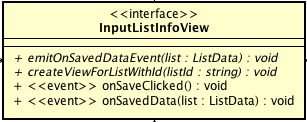
\includegraphics[scale=0.5]{Sezioni/SottosezioniST/img/app/InputListInfoView.png}
	\caption{feature::input\_list\_info::InputListInfoView}
\end{figure}

\begin{itemize}
\item \textbf{Descrizione}: Questa interfaccia rappresenta la view relativa al popup per l'immissione, rimozione o modifica di tutti i dati relativi alla lista.
\item \textbf{Utilizzo}: L'interfaccia viene utilizzata per disaccoppiare presenter e implementazione della vista, e visualizza i dati che gli vengono passati dal presenter.
\item \textbf{Attributi}: 
\item \textbf{Metodi}:
	\begin{itemize}	
	\item \textit{public emitOnSavedDataEvent(list:ListaData):void}\\
	Metodo necessario al presenter per far emettere alla view l'evento onSavedData(list:ListData), notificando tutti gli oggetti in ascolto che la lista è stata salvata con successo.
			\\ \textbf{Parametri}: \begin{itemize}
			\item \textit{list:ListaData}\\
			Insieme di tutti i dati immessi all'interno della vista da parte dell'utente.
			\end{itemize} 
	\item \textit{public createViewForListWithId(listId:string):void}\\
	Metodo che permette di creare una una view per visualizzarli.
			\\ \textbf{Parametri}: \begin{itemize}
			\item \textit{listId:string}\\
			Parametro che rappresenta l'id della lista di cui si vuole creare in una view.
			\end{itemize} 
	\end{itemize}
\item \textbf{Eventi}:
	\begin{itemize}
	\item \textit{public onSaveClicked():void}\\
	Evento emesso dalla view che rappresenta interazione di un utente con un bottone dedicato al salvataggio della lista.
	\item \textit{public onSavedData(list:ListData):void}\\
			Evento che notifica tutti gli oggetti in ascolto che i dati immessi sono stati salvati con successo.
			\\ \textbf{Parametri}: \begin{itemize}
			\item \textit{list:ListData}\\
			Insieme di tutti i dati e le informazioni di una lista.
			\end{itemize} 
	\end{itemize}
\end{itemize}

\subsubsection{feature::input\_list\_info::view::InputListInfoViewImpl}

\label{feature::input_list_info::view::InputListInfoViewImpl}
\begin{figure}[H]
	\centering
	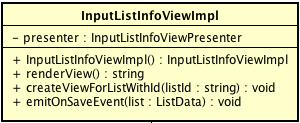
\includegraphics[scale=0.5]{Sezioni/SottosezioniST/img/app/InputListInfoViewImpl.png}
	\caption{feature::input\_list\_info::view::InputListInfoViewImpl}
\end{figure}

\begin{itemize}
\item \textbf{Descrizione}: Classe dedicata alla visualizzazione del popup che permette all'utente di inserire i dati relativi ad una lista.
\item \textbf{Utilizzo}: Classe utilizzata per visualizzare popup che permette all'utente di inserire o modificare tutti i dati relativi ad una lista.
\item \textbf{Attributi}: 
	\begin{itemize}
	\item \textit{private presenter:InputListInfoViewPresenter}\\
		Il presenter associato alla view del popup, al quale questa classe delega la gestione del comportamento della view stessa.
	\end{itemize}
\item \textbf{Metodi}:
	\begin{itemize}	
	\item \textit{public renderView():string}\\
			Genera il codice HTML CSS JS necessario per visualizzare la view.
	\item \textit{public InputListInfoViewImpl():InputListInfoViewImpl}\\
	Il costruttore della classe InputListInfoViewImpl.
	\item \textit{public createViewForListWithId(listId:string):void}\\
		Metodo che permette di creare una una view per inserire i dati di una lista, andando a pre-compilare i vari campi con i dati precedentemente inseriti della lista con id dato.
			\\ \textbf{Parametri}: \begin{itemize}
			\item \textit{listId:string}\\
			Id della lista i quali dati vogliono essere utilizzati per pre-compilare i campi di inserimento della vista.
			\end{itemize} 
	\item \textit{public emitOnSaveEvent(list:ListData):void}\\
	Evento che notifica tutti gli oggetti in ascolto che è stato richiesto il salvataggio della lista.
			\\ \textbf{Parametri}: \begin{itemize}
			\item \textit{list:ListData}\\
				Insieme di tutti i dati e le informazioni di una lista.
			\end{itemize} 
	\end{itemize}
\item{Eventi}:
\end{itemize}

\subsubsection{feature::input\_list\_info::presenter::InputListInfoViewPresenter}

\label{feature::input_list_info::presenter::InputListInfoViewPresenter}
\begin{figure}[H]
	\centering
	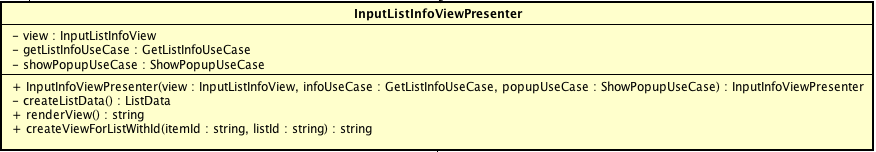
\includegraphics[scale=0.5]{Sezioni/SottosezioniST/img/app/InputListInfoViewPresenter.png}
	\caption{feature::input\_list\_info::presenter::InputListInfoViewPresenter}
\end{figure}

\begin{itemize}
\item \textbf{Descrizione}: Classe che rappresenta il presenter dedicato alla view per l'inserimento dei dati della lista.
\item \textbf{Utilizzo}: Il presenter fa da tramite tra l'implementazione della view e la parte logica dell'applicazione, formattando i dati che verranno visualizzati nella view e manipolando gli input dell'utente per eseguire le operazioni predisposte.
\item \textbf{Attributi}: 	
	\begin{itemize}
	\item \textit{private view:InputListInfoView}\\
		La view associata al presenter.
	\item \textit{private getListInfoUseCases:GetListInfoUseCases}\\
		Oggetto che permette di recuperare le informazioni di una data lista.
	\item \textit{private showPopupUseCases:ShowPopupUseCases}\\
		Oggetto che permette la creazione di un popup per l'immissione dei dati della lista da creare.	
		\end{itemize}
\item \textbf{Metodi}:
	\begin{itemize}	
	\item \textit{public InputListInfoViewPresenter(view:InputListInfoView, infoUseCase:GetListInfoUseCase, \\ popupUseCase:ShowPopupUseCase):InputListInfoViewPresenter}\\
	Il costruttore della classe InputListInfoViewPresenter.
			\\ \textbf{Parametri}: \begin{itemize}
			\item \textit{view:InputListInfoView}\\
			La view necessaria alla costruzione del presenter.
			\item \textit{infoUseCase:GetListInfoUseCase}\\
			Oggetto che permette di recuperare le informazioni di una data lista.
			\item \textit{popupUseCase:ShowPopupUseCase}\\
			Oggetto che permette la creazione di un popup per l'immissione dei dati della lista da creare.	
			\end{itemize} 
	\item \textit{private createListData():ListData}\\
	 	Metodo dedicato alla creazione dell'oggetto rappresentante l'insieme dei dati, nuovi o modificati, che compongono della lista.
	\item \textit{public renderView():string}\\
	Genera il codice HTML CSS JS necessario per visualizzare la view.
	\item \textit{public createViewForListWithId(listId:string):void}\\
		Metodo che permette di creare una una view per visualizzarli.
			\\ \textbf{Parametri}: \begin{itemize}
			\item \textit{listId:string}\\
			Parametro che rappresenta l'id della lista di cui si vuole creare in una view.
			\end{itemize} 
	\end{itemize}
\item{Eventi}:
\end{itemize}

\subsubsection{feature::change\_list\_info::ChangeListInfoView}

\label{feature::change_list_info::ChangeListInfoView}
\begin{figure}[H]
	\centering
	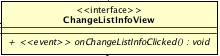
\includegraphics[scale=0.5]{Sezioni/SottosezioniST/img/app/ChangeListInfoView.png}
	\caption{feature::change\_list\_info::ChangeListInfoView}
\end{figure}

\begin{itemize}
\item \textbf{Descrizione}: Interfaccia che, una volta implementata, permette al presenter e allo sviluppatore di modificare la view dedicata alla modifica delle informazioni di una lista.
\item \textbf{Utilizzo}: L'interfaccia viene utilizzata per disaccoppiare presenter e implementazione della vista, e visualizza i dati che gli vengono passati dal presenter.
\item \textbf{Attributi}: 
\item \textbf{Metodi}:
\item{Eventi}:
	\begin{itemize}	
	\item \textit{public onChangeListInfoClicked():void}\\
		Evento che notifica tutti gli oggetti in ascolto che è stato cliccato il pulsante relativo alla modifica della lista.
	\end{itemize}
\end{itemize}

\subsubsection{feature::change\_list\_info::view::ChangeListInfoViewImpl}

\label{feature::change_list_info::view::ChangeListInfoViewImpl}
\begin{figure}[H]
	\centering
	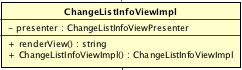
\includegraphics[scale=0.5]{Sezioni/SottosezioniST/img/app/ChangeListInfoViewImpl.png}
	\caption{feature::change\_list\_info::view::ChangeListInfoViewImpl}
\end{figure}

\begin{itemize}
\item \textbf{Descrizione}: Classe dedicata alla modifica dei dati e informazioni relativi alla lista.
\item \textbf{Utilizzo}: Il presenter fa da tramite tra l'implementazione della view e la parte logica dell'applicazione, formattando i dati che verranno visualizzati nella view e manipolando gli input dell'utente per eseguire le operazioni predisposte.
\item \textbf{Attributi}: 
	\begin{itemize}
	\item \textit{private presenter:ChangeListInfoViewPresenter}\\
	Il presenter associato alla view dedicata alla modifica dei dati relativi alla lista, al quale questa classe delega la gestione del comportamento della view stessa.
	\end{itemize}
\item \textbf{Metodi}:
	\begin{itemize}
	\item \textit{public ChangeListInfoViewImpl():ChangeListInfoViewImpl}\\
	Il costruttore della classe ChangeListInfoViewImpl.	
	\item \textit{public renderView():string}\\
	Genera il codice HTML CSS JS necessario per visualizzare la view.
	\end{itemize}
\item{Eventi}:
\end{itemize}

\subsubsection{feature::change\_list\_info::presenter::ChangeListInfoViewPresenter}

\label{feature::change_list_info::presenter::ChangeListInfoViewPresenter}
\begin{figure}[H]
	\centering
	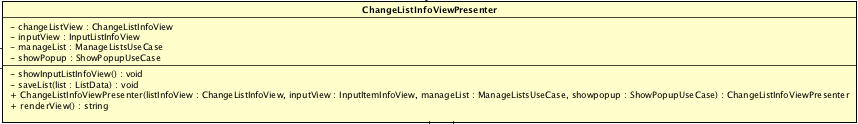
\includegraphics[scale=0.5]{Sezioni/SottosezioniST/img/app/ChangeListInfoViewPresenter.png}
	\caption{feature::change\_list\_info::presenter::ChangeListInfoViewPresenter}
\end{figure}

\begin{itemize}
\item \textbf{Descrizione}: Classe che rappresenta il presenter dedicato alla modifica delle informazioni di una lista.
\item \textbf{Utilizzo}: Il presenter fa da tramite tra l'implementazione della view e la parte logica dell'applicazione, formattando i dati che verranno visualizzati nella view e manipolando gli input dell'utente per eseguire le operazioni predisposte.
\item \textbf{Attributi}:
	\begin{itemize}
	\item \textit{private changeListView:ChangeListInfoView}\\
		La view associata al presenter.
	\item \textit{private inputView:InputListInfoView}\\
		Oggetto che rappresenta l'insieme dei dati immessi dall'utente durante la modifica della lista.
	\item \textit{private manageList:ManageListsUseCase}\\
Oggetto dedicato alla gestione dei dati relativi alla lista all'interno del database.
	\item \textit{private showPopup:ShowPopupUseCase}\\
		Oggetto che permette la creazione di un popup per l'immissione dei dati della lista da creare.	
	\end{itemize} 
\item \textbf{Metodi}:
	\begin{itemize}
	\item \textit{public ChangeListInfoViewPresenter(listInfoView:ChangeListInfoView, inputView:InputItemInfoView, \\ manageList:ManageListsUseCase, showpopup:ShowPopupUseCase):ChangeListInfoViewPresenter}\\
Il costruttore della classe ChangeListInfoViewPresenter.
			\\ \textbf{Parametri}: \begin{itemize}
			\item \textit{listInfoView:ChangeListInfoView}\\
			La view necessaria alla costruzione del presenter.
			\item \textit{inputView:InputListInfoView}\\
			Oggetto che rappresenta la vista per l'immissione dei dati relativi ad una lista.
			\item \textit{manageList:ManageListsUseCase}\\
			Oggetto dedicato alla gestione delle liste all'interno del database.
			\item \textit{showpopup:ShowPopupUseCase}\\
			Oggetto che permette la creazione di un popup per l'immissione dei dati della lista da modificare.	
			\end{itemize} 
	\item \textit{private showInputListInfoView():void}\\
		Metodo che permette di visualizzare il popup che conterrà la vista dove l'utente modificherà i dati della lista.
	\item \textit{private createViewForListWithId(listId:string):void}\\
		Metodo che permette di creare la vista per la modifica dei dati di una lista precompilando i campi di input con i dati della lista con id dato.
			\\ \textbf{Parametri}: \begin{itemize}
			\item \textit{listId:string}\\
			Id della lista i quali dati verranno utilizzati per precompilare i campi di input della vista.
			\end{itemize} 
	\item \textit{public renderView():string}\\
	Genera il codice HTML CSS JS necessario per visualizzare la view.
	\end{itemize} 
\item{Eventi}:
\end{itemize}

\subsubsection{usecase::GetListInfoUseCase}

\label{usecase::GetListInfoUseCase}
\begin{figure}[H]
	\centering
	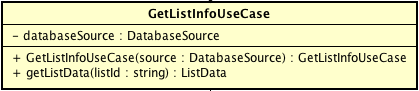
\includegraphics[scale=0.5]{Sezioni/SottosezioniST/img/app/GetListInfoUseCase.png}
	\caption{usecase::GetListInfoUseCase}
\end{figure}

\begin{itemize}
\item \textbf{Descrizione}: 
\item \textbf{Utilizzo}:
\item \textbf{Attributi}: 
	\begin{itemize}
	\item \textit{private databaseSource:DatabaseSource}\\
		Riferimento al database.
	\end{itemize}
\item \textbf{Metodi}:
	\begin{itemize}
	\item \textit{GetListInfoUseCase(source:DatabaseSource):GetListInfoUseCase}\\
	Il costruttore della classe GetListInfoUseCase.
			\\ \textbf{Parametri}: \begin{itemize}
			\item \textit{source:DatabaseSource}\\
		Riferimento al database.
			\end{itemize}
	\item \textit{public getListData(listId:string):ListData}\\
	Metodo che restituisce l'insieme dei dati e informazioni relativi a una lista.
				\\ \textbf{Parametri}: \begin{itemize}
				\item \textit{listId:string}\\
				Parametro che rappresenta l'id della lista di cui si vuole recuperare i dati e le informazioni.
				\end{itemize} 
	\end{itemize}
\item{Eventi}:
\end{itemize}